
\subsection{Recording}
There are several approaches to assemble components to achieve a recording, and we review an alternative structure. In Figure \ref{fig:hta_recording} we have an HTA graph, which illustrate the building blocks to enable a recording and their dependencies:

\begin{figure}
    \centering
    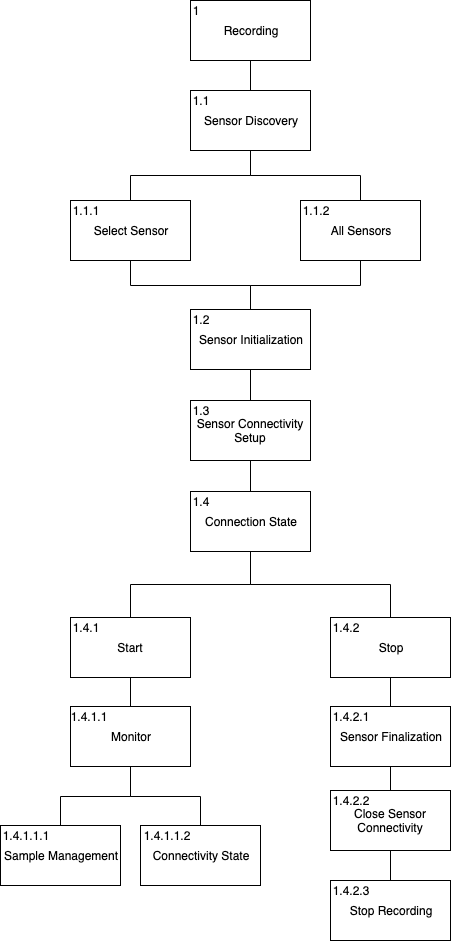
\includegraphics[width=0.65\textwidth]{images/Recording.png}
    \caption{Recording}
    \label{fig:hta_recording}
\end{figure}

\begin{itemize}
    \item Sensor Discover: Has to find all eligible sensors that can enable a recording.
    \item Select Sensors: From the sensor discovery, we can choose preferable sensors sources.
    \item  All Sensors: More straightforward, we sample from all of the available sensors.
    \item Sensor Initialization: Once we have a list of sensors sources, we need to establish and initialize a connection with the sensors. Occasionally a sensor might use some time to connect, or unforeseen occurrence is hindering the initialization of the sensor. Thus, blocking the state of the recording. 
    \item Sensor Connectivity Setup: Additionally, we establish a connection between the application and the sensor source. All data exchange occurs over the established interface. 
    \item Connection Stat: Based on sensors establishments we can proceed to either start or stop a recording. 
    \item Start: By starting, we notify the sensors to begin collecting data, and the view should display that a recording has begun accordingly.
    \item Monitor: Is continuously waiting for new samples to arrive on the interface defined between the application and the sensors.
    \item Sample Management: Once a new sample has arrived, we need to store the sample on a persistent storage.
    \item Connectivity State: If it is an external sensor, the sensor source might disconnect during a recording. Thus, implementing a mechanism to check for continuous data stream is a critical task.
    \item Stop: By stopping, we notify the sensors to stop collecting data from the sensor source.
    \item Sensor Finalization: We notify the sensor to stop sampling data, and close establishment.
    \item Close Sensor Connectivity: We close the interface establishment between the application and the sensors. 
    \item Stop Recording: Once the sensors has closed its connections, we can add additional information to the recording (e.g., title, description, rating). In the end, the recording has concluded and its stored on the mobile device.

\end{itemize}

This suggested structure of a recording is one alternative to enable a recording. Most of the components suggested in the structure are essential to a recording. A naive solution would be to ignore the connectivity state component, by assuming the sensors are connected indefinitely. In our thesis, we will be following 


\subsection{Sharing}

\subsection{Modules}

\subsection{Storage}

\subsection{Presentation}
